\documentclass[paper=a4, fontsize=11pt]{scrartcl} 

\usepackage[T1]{fontenc} 
\usepackage[english]{babel}
\usepackage{amsmath,amsfonts,amsthm}

\usepackage{lipsum}

\usepackage{graphicx}
\usepackage{float}
  \floatplacement{figure}{H}
  \floatplacement{table}{H}
  
\usepackage{sectsty} 
\allsectionsfont{\centering \normalfont\scshape} 

\usepackage{fancyhdr} % Custom headers and footers
\pagestyle{fancyplain} % Makes all pages in the document conform to the custom headers and footers
\fancyhead{} % No page header - if you want one, create it in the same way as the footers below
\fancyfoot[L]{} % Empty left footer
\fancyfoot[C]{} % Empty center footer
\fancyfoot[R]{\thepage} % Page numbering for right footer
\renewcommand{\headrulewidth}{0pt} % Remove header underlines
\renewcommand{\footrulewidth}{0pt} % Remove footer underlines
\setlength{\headheight}{13.6pt} % Customize the height of the header

\usepackage[labelformat=empty]{caption}
\usepackage{color}
\usepackage{listings}
\lstset{ %
language=bash,                % choose the language of the code
basicstyle=\footnotesize,       % the size of the fonts that are used for the code
numbers=left,                   % where to put the line-numbers
numberstyle=\footnotesize,      % the size of the fonts that are used for the line-numbers
stepnumber=1,                   % the step between two line-numbers. If it is 1 each line will be numbered
numbersep=5pt,                  % how far the line-numbers are from the code
backgroundcolor=\color{white},  % choose the background color. You must add \usepackage{color}
showspaces=false,               % show spaces adding particular underscores
showstringspaces=false,         % underline spaces within strings
showtabs=false,                 % show tabs within strings adding particular underscores
frame=single,           % adds a frame around the code
tabsize=2,          % sets default tabsize to 2 spaces
captionpos=b,           % sets the caption-position to bottom
breaklines=true,        % sets automatic line breaking
breakatwhitespace=false,    % sets if automatic breaks should only happen at whitespace
escapeinside={\%*}{*)}          % if you want to add a comment within your code
}



\numberwithin{equation}{section} % Number equations within sections (i.e. 1.1, 1.2, 2.1, 2.2 instead of 1, 2, 3, 4)
\numberwithin{figure}{section} % Number figures within sections (i.e. 1.1, 1.2, 2.1, 2.2 instead of 1, 2, 3, 4)
\numberwithin{table}{section} % Number tables within sections (i.e. 1.1, 1.2, 2.1, 2.2 instead of 1, 2, 3, 4)

\setlength\parindent{0pt} % Removes all indentation from paragraphs - comment this line for an assignment with lots of text

%----------------------------------------------------------------------------------------
%	TITLE SECTION
%----------------------------------------------------------------------------------------

\newcommand{\horrule}[1]{\rule{\linewidth}{#1}} % Create horizontal rule command with 1 argument of height

\title{	
\normalfont \normalsize 
\textsc{Computational Science - ITB} \\ [25pt] % Your university, school and/or department name(s)
\horrule{0.5pt} \\[0.4cm] % Thin top horizontal rule
\small Algoritma dan Desain Perangkat Lunak\\
\large Desain Sistem Pelaporan Akademik: \textit{Waterfall model} \\ % The assignment title
%\horrule{2pt} \\[0.5cm] % Thick bottom horizontal rule
}

\author{\small Febrie Ahmad A. || 20912008 \\ \small Ridlo W. Wibowo || 20912009} % Your name

\date{\normalsize\today} % Today's date or a custom date

\begin{document}

\maketitle % Print the title

\large \textbf{System Requirement and Analysis}
\begin{itemize}
\item \textbf{Introduction}
	\begin{itemize}
	\item \textit{Purpose}: sistem yang memberikan informasi mengenai kondisi studi mahasiswa.
	\item \textit{System overview}: sistem dapat memberikan informasi ke berbagai pihak terkait studi mahasiswa sesuai hubungannya dengan mahasiswa.
	\item \textit{External Entity}: Sistem Keuangan, Sistem Akademik, Sistem Lembaga Kemahasiswaan, Mahasiswa, Orang Tua/Wali, Dosen Wali, Ketua Program Studi, Karyawan Tata Usaha.
	\end{itemize}
\item \textbf{Overall description}
	\begin{itemize}
	\item \textit{Product perspective}\\
		\textit{User Interfaces}: memberikan informasi melalui media website untuk mahasiswa, dosen wali, kaprodi, dan karyawan TU.\\
		\textit{Communication Interfaces}: memberikan informasi dan peringatan melalui post, pesan singkat dan email.
	\item \textit{User characteristics}\\
		\textit{Mahasiswa}: bisa menggunakan media internet, manajemen waktu masih buruk sehingga diperlukan pengingat.\\
		\textit{Orang Tua}: biasanya tidak mahir menggunakan media internet, membutuhkan laporan akademik anaknya, juga laporan keuangan dan apabila terjadi kasus.\\
		\textit{Dosen Wali}: bisa menggunakan media internet, membutuhkan informasi akademik mahasiswa perwaliannya.\\
		\textit{Ketua Prodi}: bisa menggunakan media internet, membutuhkan informasi akademik mahasiswa progam studinya untuk keperluan pengawasan.\\
		\textit{Karyawan TU}: bisa menggunakan media internet, membutuhkan informasi akademik mahasiswa program studi untuk keperluan bantuan print dan pelaporan.\\
	\item \textit{Constraints, assumptions and dependencies}\\
		\textit{constraints}: pelaporan hanya meliputi mata kuliah (yang harus diambil, belum diambil dan sudah diambil), nilai, kasus akademik, nonakademik dan keuangan.\\
		\textit{assumptions}: telah ada sistem pendukung yang butuhkan, kantor pos sudah menggunakan teknologi yang dibutuhkan.\\
		\textit{dependencies}: sistem akademik, sistem keuangan, dan sistem lembaga kemahasiswaan.
	\end{itemize}
\item \textbf{Specific requirements}
	\begin{itemize}		
	\item \textit{External interface requirements}
	\begin{itemize}
		\item SMS Gateway.
		\item Post Gateway.
		\item Koneksi jaringan ke sistem yang lain.
	\end{itemize}

	\item \textit{Functional requirements}: web service untuk masing-masing user sesuai kebutuhannya.
	\item \textit{Performance requirements}
	\begin{itemize}
		\item dapat diakses ribuan orang sekali waktu.
		\item aman, terutama menyangkut nilai studi mahasiswa.
	\end{itemize}
	\end{itemize}
\end{itemize}		
		

\newpage
\large \textbf{Context Diagram}
\begin{figure}
	\centering
	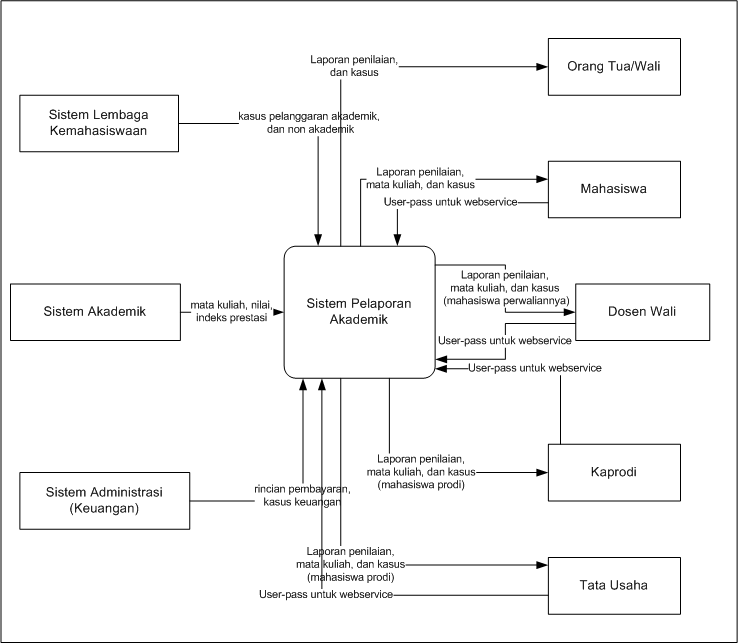
\includegraphics[width=0.9\textwidth]{diagramkonteksSPA.png}
	\caption{Diagram Konteks.}
\end{figure}

\newpage
\large \textbf{Data Flow Diagram}\\
\textit{level 0}


\end{document}














